\documentclass{article}

% The style file is the unmodified neurips_2025.sty from the course link:
% https://media.neurips.cc/Conferences/NeurIPS2025/Styles.zip
% Preprint mode displays the author line without claiming conference acceptance.
\usepackage[preprint,nonatbib]{neurips_2025}
\usepackage{graphicx}
\usepackage{url}
\urlstyle{same}

\title{Generating Chest Radiographs with a Convolutional Variational Autoencoder}
\author{ECE 285 Homework 1}

\begin{document}
\maketitle

\begin{abstract}
We train one convolutional variational autoencoder (VAE) on the Chest X-Ray
Images (Pneumonia) training split after reserving a stratified validation
subset, then draw unconditional samples from its Gaussian prior. We report
training behavior, example radiographs, Inception
Score (IS), and an explicitly identified 1000-feature Fr\'echet Inception
Distance (FID-1000). The generated images capture coarse chest structure but
blur fine anatomy; these natural-image metrics do not establish diagnostic
quality.
\end{abstract}

\section{Data and method}
We use the Kaggle pediatric chest X-ray dataset~\cite{mooney}. The original
training split is stratified into 4,694 training and 522 validation images
(seed 285); the separate 624-image test split is reserved for evaluation.
One VAE covers both NORMAL and PNEUMONIA images. Images are converted to
grayscale, resized to $64\times64$, and scaled to $[0,1]$.

Four stride-two convolutional encoder layers produce $4\times4\times128$
features. Linear heads parameterize a 32-dimensional diagonal Gaussian
posterior; a reparameterized sample enters a linear layer and four transposed
convolutions ending in a sigmoid. The model has 543,649 trainable parameters.
Following Kingma and Welling~\cite{kingma}, we minimize per-image pixelwise
binary cross-entropy (summed over pixels) plus
$\beta D_{\mathrm{KL}}[q_\phi(z\mid x)\Vert\mathcal N(0,I)]$, with $\beta=1$.
At generation time, $z\sim\mathcal N(0,I)$; no test image is supplied.

\section{Training}
We train with Adam (learning rate $10^{-3}$), batch size 64, for 20 epochs on
CPU. The checkpoint is selected by minimum validation negative ELBO. The test
split does not enter training or checkpoint selection. At epoch 20, the best
validation loss is 2,388.10 nats/image (reconstruction 2,365.96; KL 22.14);
the final training loss is 2,397.53. Figure~\ref{fig:loss} shows the loss
trend.

\begin{figure}[t]
  \centering
  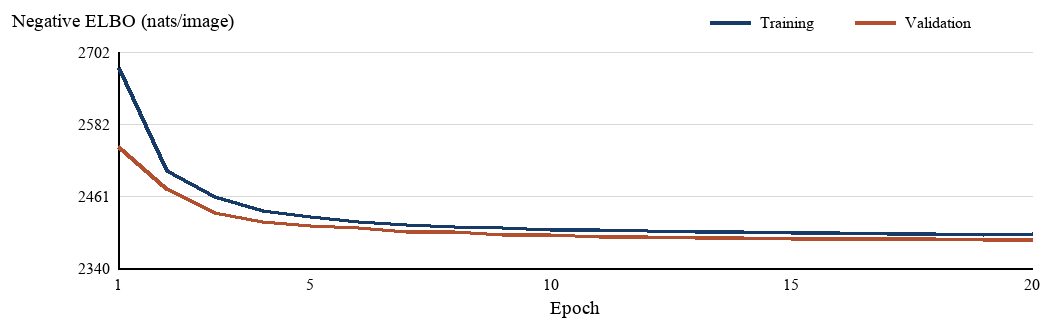
\includegraphics[width=0.86\linewidth]{results/loss_curve.png}
  \caption{Mean negative ELBO in nats/image on training and validation splits;
  lower is better. The selected checkpoint is epoch 20.}
  \label{fig:loss}
\end{figure}

\section{Generative evaluation}
We compare 256 independent prior samples with 256 randomly chosen official
test images. For Ignite's IS and FID implementation~\cite{ignite}, each
grayscale image is repeated to RGB, resized to $299\times299$, and evaluated
by ImageNet-pretrained Inception-v3. The scores are IS $=1.779$ and
FID-1000 $=0.177$. FID-1000 uses the model's 1000-class probabilities as
features, as in the cited Ignite tutorial; it is not comparable to the usual
pool3/2048-feature FID~\cite{heusel}. The sample count is small, and an
ImageNet classifier is not calibrated to radiographic anatomy.

\begin{figure}[t]
  \centering
  \begin{minipage}{0.42\linewidth}
    \centering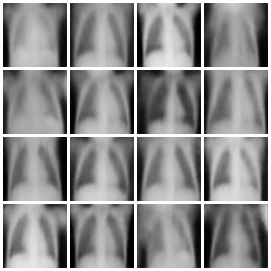
\includegraphics[width=\linewidth]{results/generated_grid.png}
    \centerline{(a) Prior samples}
  \end{minipage}\hfill
  \begin{minipage}{0.42\linewidth}
    \centering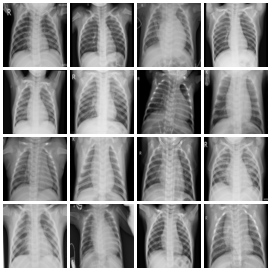
\includegraphics[width=\linewidth]{results/real_grid.png}
    \centerline{(b) Held-out test images}
  \end{minipage}
  \caption{Generated and real $64\times64$ grayscale radiographs displayed
  at the same scale. The model recovers coarse chest outlines but loses rib
  and lung texture.}
  \label{fig:examples}
\end{figure}

\section{Discussion}
Figure~\ref{fig:examples} shows visibly smoother generated images than real
test images. Downsampling removes fine lung detail, and pixelwise binary
cross-entropy with a compact Gaussian latent model can favor smooth outputs.
The training set is class-imbalanced; this unconditional model cannot select
pathology. IS and FID-1000 describe only this specific 256-sample experiment,
not clinical realism or diagnostic performance. Higher resolution and
radiology-specific evaluation would be useful next steps.

\noindent\textbf{Code and reproducibility:}
\url{https://github.com/Tobudase/ece285-hw1-chest-xray-vae}.

\small
\begin{thebibliography}{4}
\bibitem{mooney} P. Mooney. Chest X-Ray Images (Pneumonia). Kaggle, 2018.
\url{https://www.kaggle.com/datasets/paultimothymooney/chest-xray-pneumonia}.
\bibitem{kingma} D. P. Kingma and M. Welling. Auto-Encoding Variational Bayes. ICLR, 2014.
\bibitem{ignite} PyTorch-Ignite. GAN evaluation using FID and IS.
\url{https://pytorch-ignite.ai/blog/gan-evaluation-with-fid-and-is/}.
\bibitem{heusel} M. Heusel et al. GANs Trained by a Two Time-Scale Update Rule
Converge to a Local Nash Equilibrium. NeurIPS, 2017.
\end{thebibliography}

\end{document}
